\chapter{Uncertainty, Time Evolution, and the Classical Limit}

This lecture begins with a deliberate detour, returns to the wave function as the central object, proves the uncertainty principle in a stripped-down but revealing form, and only then comes back to the Schr\"odinger equation itself. The order matters. We are not given a bag of formulas; we are shown why each one is wanted. These notes follow Leonard Susskind's lecture closely, and where the blackboard layout matters the preserved board frames curated by LazyingArt LLC and Video2Book are kept in place.

\section{A Brief Detour: Negative Energy and Dirac's Idea}

Susskind opens by revisiting the toy Hamiltonian
\begin{equation}
H=cP.
\end{equation}
For momentum eigenstates the corresponding wave functions are plane waves,
\begin{equation}
\psi_p(x)=e^{ipx}.
\end{equation}
There is nothing mathematically defective about positive or negative \(p\). Both signs give perfectly acceptable plane waves. But with \(H=cP\), the sign of the momentum is also the sign of the energy. That is the difficulty.

If negative-energy particles were allowed in ordinary empty space, then empty space would not be the lowest-energy state. One could always lower the energy by adding more negative-energy particles while balancing the bookkeeping with positive-energy radiation. The qualitative conclusion is that a stable world requires the vacuum to be the lowest-energy state.

The lecture resolves this only as a physical aside, not as a full formal construction. Dirac's idea works for fermions: if negative-energy states are all filled, then Pauli exclusion prevents us from piling more particles into the same states. In that sense the vacuum is already full of all negative-energy fermion states, and no further decay is possible. The same trick fails for bosons, because bosons can pile into the same state without limit. So the opening model can be thought of as a useful baby version of the Dirac story for fermions, but not as a general theory of bosons.

This is where Susskind closes the detour. The point is not to build relativistic quantum field theory here. The point is to clear one conceptual debt and then return to the main subject of the lecture.

\section{Wave Functions, Representations, and Many Coordinates}

The bridge back to the advertised topic is the wave function. In position space,
\begin{equation}
\psi(x)=\langle x|\psi\rangle,
\end{equation}
the amplitude that the state \(|\psi\rangle\) be found at the position \(x\). In momentum space we have the same state projected onto momentum eigenstates,
\begin{equation}
\tilde{\psi}(p)=\langle p|\psi\rangle.
\end{equation}
The two are related by Fourier transform. In the one-dimensional setting of the lecture we may write
\begin{equation}
\psi(x)=\frac{1}{\sqrt{2\pi}}\int dp\,\tilde{\psi}(p)e^{ipx}.
\end{equation}
Susskind does not stop to emphasize transform conventions; the point here is qualitative and structural. A narrow profile in one representation is accompanied by a broad profile in the conjugate one.

The discussion then widens for a moment. If a particle can move in more than one spatial direction, then its position is described by several coordinates. The important point is that different spatial coordinates commute. That is not a purely formal consequence of earlier axioms; Susskind emphasizes that it is an empirical fact about the way quantum mechanics matches experiment. Thus in more than one dimension the wave function depends on all the commuting coordinates at once.

The same is true, more strongly, for several particles. The wave function of a many-particle system is a function of all the coordinates of all the particles. One may also use mixed representations, leaving some variables in coordinate space and others in momentum space. But for the rest of the lecture we return to one-dimensional motion, where the essential issues can be displayed without drowning in notation.

\section{From Noncommutation to a Definition of Uncertainty}

The uncertainty principle first appears in the lecture in its most primitive form. Position and momentum do not commute, so they do not possess simultaneous sharp eigenstates. Position eigenstates are sharply localized; momentum eigenstates are plane waves extending across all space. From Fourier analysis alone one sees the pattern: the narrower a function is in \(x\), the broader its transform is in \(p\), and vice versa.

\subsection{Question \& Answer}

Why does the lecture first shift the origin so that \(\langle X\rangle=0\)? Because Susskind wants a width, not a location. The center of a distribution can be moved by a mere change of coordinates. What should remain after this shift is the spread of the distribution around that center. In that shifted frame, the uncertainty is simply the expectation value of the square.

\begin{definition}
After shifting the origin so that \(\langle X\rangle=0\), the squared uncertainty in position is defined by
\begin{equation}
(\Delta x)^2=\langle X^2\rangle.
\end{equation}
More generally, without shifting the origin, one uses the variance
\begin{equation}
(\Delta x)^2=\langle X^2\rangle-\langle X\rangle^2.
\end{equation}
\end{definition}

In position space this becomes
\begin{equation}
(\Delta x)^2=\int dx\,\psi^*(x)\psi(x)\,x^2.
\end{equation}
This is a natural measure of width: the farther probability is spread from the origin, the larger \(\langle X^2\rangle\) becomes.

\begin{figure}
\centering

\includegraphics[width=0.78\textwidth]{lecture_10_figure_02.png}
\caption{Position uncertainty written as an integral over probability density.}
\end{figure}

\begin{figure}
\centering
\begin{tikzpicture}[x=1cm,y=1cm]
\draw[->] (-4.2,0) -- (4.2,0);
\draw[->] (0,0) -- (0,2.5);
\draw[smooth] plot coordinates {(-3.5,0.02) (-2.7,0.10) (-2.0,0.35) (-1.4,0.90) (-0.9,1.55) (-0.4,2.00) (0,2.15) (0.4,2.00) (0.9,1.55) (1.4,0.90) (2.0,0.35) (2.7,0.10) (3.5,0.02)};
\draw[dashed] (0,0) -- (0,2.15);
\node at (0,-0.35) {\(x=0\)};
\node at (2.8,2.05) {\(|\psi(x)|^2\)};
\end{tikzpicture}
\caption{A wave packet after shifting the origin so that its center is at \(\langle X\rangle=0\).}
\end{figure}

Momentum uncertainty is defined in the same spirit. One could write, in momentum space,
\begin{equation}
(\Delta p)^2=\int dp\,|\tilde{\psi}(p)|^2\,p^2,
\end{equation}
again after shifting so that \(\langle P\rangle=0\). But the lecture immediately prefers to rewrite this in the position representation, because that will let the proof proceed with both uncertainties written in one common language.

\section{Proving the Uncertainty Principle}

The first step is to remember how the momentum operator acts in the \(x\)-representation:
\begin{equation}
P=-i\,\partial_x,
\qquad
P^2=-\partial_x^2.
\end{equation}
Therefore
\begin{equation}
(\Delta p)^2=\langle \psi|P^2|\psi\rangle
=-\int dx\,\psi^*(x)\,\partial_x^2\psi(x).
\end{equation}

\subsection{Question \& Answer}

How can \((\Delta p)^2\) be positive when the first \(x\)-space formula carries a minus sign? The answer is that the integral itself is negative. One sees this by integration by parts:
\begin{equation}
\int f\,g'\,dx=-\int f' g\,dx,
\end{equation}
provided the boundary term vanishes. For a normalizable wave function, \(\psi(x)\) goes to zero at infinity, so this is the rule we use.

Applying it once gives
\begin{equation}
(\Delta p)^2
=\int dx\,\bigl(\partial_x\psi^*(x)\bigr)\bigl(\partial_x\psi(x)\bigr),
\end{equation}
which is manifestly nonnegative.

The board at this stage is worth preserving because it shows the architecture of the proof: the position variance, the momentum variance rewritten in \(x\)-space, and on the right the vector inequality that will tie them together.

\begin{figure}
\centering

\includegraphics[width=0.88\textwidth]{lecture_10_figure_03.png}
\caption{Variance formulas beside the vector-space inequality.}
\end{figure}

In cleaned Hilbert-space notation, the inequality we want is
\begin{equation}
\langle A|A\rangle\,\langle B|B\rangle \ge |\langle A|B\rangle|^2.
\end{equation}
Susskind calls this the triangle inequality in vector-space language; in polished form it is the Cauchy-Schwarz inequality.

\begin{figure}
\centering
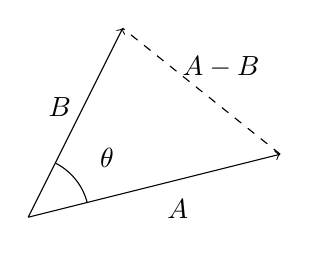
\begin{tikzpicture}[x=1cm,y=1cm]
\draw[->] (0,0) -- (3.2,0.8);
\draw[->] (0,0) -- (1.2,2.4);
\draw[dashed] (3.2,0.8) -- (1.2,2.4);
\node at (1.9,0.1) {\(A\)};
\node at (0.4,1.4) {\(B\)};
\node at (2.45,1.9) {\(A-B\)};
\draw (0.75,0.18) arc[start angle=14,end angle=63,radius=0.78];
\node at (1.0,0.75) {\(\theta\)};
\end{tikzpicture}
\caption{The geometric picture behind the inequality Susskind invokes: the dot product is bounded by the product of lengths.}
\end{figure}

The proof now becomes a clever choice of vectors. We define
\begin{equation}
|A\rangle=X|\psi\rangle,
\qquad
|B\rangle=P|\psi\rangle.
\end{equation}
In the position representation this means
\begin{equation}
A(x)=x\psi(x),
\qquad
B(x)=-i\,\frac{d\psi}{dx}.
\end{equation}
At this point the lecture introduces one simplifying assumption: to keep the algebra on the blackboard under control, take \(\psi(x)\) to be real. The general proof is not conceptually different, but it requires carrying \(\psi^*\) through more lines.

\begin{figure}
\centering

\includegraphics[width=0.84\textwidth]{lecture_10_figure_04.png}
\caption{Choice of \(A\) and \(B\) for the uncertainty proof.}
\end{figure}

\begin{theorem}
In the simplified proof where \(\langle X\rangle=\langle P\rangle=0\), \(\psi(x)\) is taken real, and \(\hbar=1\), the uncertainty product satisfies
\begin{equation}
\Delta x\,\Delta p \ge \frac{1}{2}.
\end{equation}
\end{theorem}

\begin{proof}
With the above definitions,
\begin{equation}
\langle A|A\rangle=(\Delta x)^2,
\qquad
\langle B|B\rangle=(\Delta p)^2.
\end{equation}
Therefore
\begin{equation}
(\Delta x)^2(\Delta p)^2 \ge |\langle A|B\rangle|^2.
\end{equation}
Now
\begin{equation}
|\langle A|B\rangle|^2
=
\left|
\int dx\,\psi(x)\,x\,\frac{d\psi}{dx}
\right|^2,
\end{equation}
where the overall sign and factor of \(i\) are irrelevant inside the absolute value.

Because \(\psi\) is real in this simplified proof,
\begin{equation}
\psi\,\frac{d\psi}{dx}
=
\frac{1}{2}\frac{d}{dx}\bigl(\psi^2\bigr).
\end{equation}
So
\begin{equation}
\int dx\,\psi(x)\,x\,\frac{d\psi}{dx}
=
\frac{1}{2}\int dx\,x\,\frac{d}{dx}\bigl(\psi^2\bigr).
\end{equation}
Integrating by parts and using \(\frac{d}{dx}x=1\), together with the vanishing boundary term, we obtain
\begin{equation}
\frac{1}{2}\int dx\,x\,\frac{d}{dx}\bigl(\psi^2\bigr)
=
-\frac{1}{2}\int dx\,\psi^2.
\end{equation}
For a normalized state,
\begin{equation}
\int dx\,\psi^2=1,
\end{equation}
so
\begin{equation}
|\langle A|B\rangle|^2=\frac{1}{4}.
\end{equation}
Hence
\begin{equation}
(\Delta x)^2(\Delta p)^2 \ge \frac{1}{4},
\end{equation}
and taking square roots gives
\begin{equation}
\Delta x\,\Delta p \ge \frac{1}{2}.
\end{equation}
Restoring units,
\begin{equation}
\Delta x\,\Delta p \ge \frac{\hbar}{2}.
\end{equation}
\end{proof}

\begin{figure}
\centering

\includegraphics[width=0.84\textwidth]{lecture_10_figure_05.png}
\caption{The boxed uncertainty bound at the end of the proof.}
\end{figure}

\subsection{Question \& Answer}

Why is the final statement really \(\ge\), and when can equality occur? Susskind himself is corrected on this point in the lecture. The distinction is not cosmetic. If the inequality were not sharp, a stronger bound might still be waiting to be proved. But in this case equality can in fact be attained. There are wave packets for which
\begin{equation}
\Delta x\,\Delta p=\frac{\hbar}{2},
\end{equation}
and those are the minimal uncertainty packets to which the next lecture will turn.

\begin{remark}
The board frame shows a strict sign, but the mathematically correct statement is the non-strict inequality. The lecture explicitly acknowledges this.
\end{remark}

\section{After the Proof: Minimal Packets and Other Conjugate Pairs}

The proof does not end the discussion. Susskind lets several loose ends breathe.

First, the boundary term in integration by parts vanishes because a normalizable wave function must decay at infinity. This is not a decorative assumption; it is what turns the formal manipulations into honest identities.

Second, the inequality is tight. The existence of wave packets that saturate the bound means the theorem has real content. One does not merely know that \(\Delta x\,\Delta p\) is not too small; one knows the best possible lower bound.

Third, position and momentum are not the only conjugate pair in town. The time dependence of a wave function may be written schematically as a Fourier expansion in energy,
\begin{equation}
\psi(t)\sim \int dE\,\phi(E)e^{-iEt}.
\end{equation}
This is enough for the lecture's qualitative point: if two descriptions are related by Fourier transform, then narrowing one tends to broaden the other. In that sense there is also a time-energy uncertainty relation. Susskind is careful, however, not to turn this into a full formal theorem in the present lecture. The usage is subtler.

The same broad pattern holds for angle and angular momentum. If a rotating body is described by an angle \(\theta\), then \(\theta\) and the corresponding angular momentum form another conjugate pair. The lecture keeps this at the level of analogy, and so should we.

\section{The Schr\"odinger Equation in Abstract and in Position Space}

Only now does Susskind say, in effect, let us return to the real business of the day. The abstract law of time evolution is
\begin{equation}
i\,\frac{d}{dt}|\psi\rangle = H|\psi\rangle.
\end{equation}
He then chooses the most familiar Hamiltonian for a one-dimensional particle in a potential,
\begin{equation}
H=\frac{P^2}{2m}+V(X).
\end{equation}
This is the quantized version of the classical particle Hamiltonian. The lecture is frank about the logic: one lifts the classical expression into quantum mechanics and then checks afterward whether the resulting wave-packet motion matches classical expectations when it ought to.

\begin{figure}
\centering

\includegraphics[width=0.76\textwidth]{lecture_10_figure_06.png}
\caption{The board reset as the lecture returns to abstract time evolution.}
\end{figure}

In the \(x\)-representation we replace \(P\) by \(-i\partial_x\), so
\begin{equation}
i\,\partial_t\psi(x,t)
=
-\frac{1}{2m}\partial_x^2\psi(x,t)+V(x)\psi(x,t).
\end{equation}
Susskind also writes the complex conjugate equation because both forms will be used in the expectation-value derivations:
\begin{equation}
\partial_t\psi^*(x,t)
=
-\frac{i}{2m}\partial_x^2\psi^*(x,t)+iV(x)\psi^*(x,t).
\end{equation}

\subsection{Question \& Answer}

What does it mean for \(V(x)\) to be an operator? In this representation the answer is almost embarrassingly simple: it multiplies the wave function. The operator \(X\) multiplies by \(x\); a function of \(X\) multiplies by the corresponding function. Thus
\begin{equation}
V(X)\psi(x)=V(x)\psi(x).
\end{equation}
Susskind pauses over this because it is a definition, and definitions in physics are not given for free. They earn their place by leading to useful equations. Here the test will be whether they reproduce the correct motion of expectation values.

\section{Expectation Values, Ehrenfest-Type Equations, and the Limits of Classical Motion}

The next goal is to see how the center of a wave packet moves. If a packet remains reasonably localized, its center may be identified with the expectation value of position. We therefore ask for the time dependence of \(\langle X\rangle\) and \(\langle P\rangle\).

\begin{proposition}
For the Hamiltonian \(H=\frac{P^2}{2m}+V(X)\),
\begin{equation}
\frac{d}{dt}\langle X\rangle=\frac{\langle P\rangle}{m}.
\end{equation}
\end{proposition}

\begin{proof}
Start from
\begin{equation}
\langle X\rangle=\int dx\,\psi^*(x,t)\,x\,\psi(x,t).
\end{equation}
Differentiating with respect to time gives two terms,
\begin{equation}
\frac{d}{dt}\langle X\rangle
=
\int dx\,\dot{\psi}^*\,x\,\psi
+
\int dx\,\psi^*\,x\,\dot{\psi}.
\end{equation}
These are complex conjugates, so it is enough to keep one and add its conjugate at the end. Substituting the conjugate Schr\"odinger equation into the first term, the contribution proportional to \(V(x)\) is pure imaginary and cancels against its conjugate. What remains comes from the kinetic term. After one integration by parts, the derivative hits \(x\) and produces \(1\), while the remaining term is purely imaginary and drops out from the final real answer. The result is
\begin{equation}
\frac{d}{dt}\langle X\rangle
=
\frac{1}{m}\int dx\,\psi^*(-i\partial_x)\psi
=
\frac{\langle P\rangle}{m}.
\end{equation}
\end{proof}

This is one half of mechanics: velocity equals momentum divided by mass.

\begin{proposition}
For the same Hamiltonian,
\begin{equation}
\frac{d}{dt}\langle P\rangle=-\left\langle \frac{dV}{dx}\right\rangle.
\end{equation}
\end{proposition}

\begin{proof}
Write the expectation value of momentum as
\begin{equation}
\langle P\rangle=\int dx\,\psi^*(-i\partial_x)\psi.
\end{equation}
Differentiate with respect to time:
\begin{equation}
\frac{d}{dt}\langle P\rangle
=
-i\int dx\,\dot{\psi}^*\,\partial_x\psi
-i\int dx\,\psi^*\,\partial_x\dot{\psi}.
\end{equation}
One rearranges the second term by integration by parts so that the pair can be compared by complex conjugation. Substituting the Schr\"odinger equations for \(\dot{\psi}\) and \(\dot{\psi}^*\), the kinetic contribution reduces to a purely imaginary quantity and therefore does not survive in the final real answer.

The potential contribution is the interesting part. It combines into
\begin{equation}
\int dx\,V(x)\bigl(\psi\,\partial_x\psi^*+\psi^*\,\partial_x\psi\bigr).
\end{equation}
But the bracket is just the derivative of the probability density:
\begin{equation}
\psi\,\partial_x\psi^*+\psi^*\,\partial_x\psi
=
\partial_x\bigl(\psi^*\psi\bigr).
\end{equation}
So we arrive at
\begin{equation}
\frac{d}{dt}\langle P\rangle
=
\int dx\,V(x)\,\partial_x\bigl(\psi^*\psi\bigr).
\end{equation}
Integrating by parts once more gives
\begin{equation}
\frac{d}{dt}\langle P\rangle
=
-\int dx\,\psi^*(x,t)\psi(x,t)\,\frac{dV}{dx},
\end{equation}
or, in expectation-value notation,
\begin{equation}
\frac{d}{dt}\langle P\rangle=-\left\langle \frac{dV}{dx}\right\rangle.
\end{equation}
\end{proof}

If we define the force by
\begin{equation}
F(x)=-\frac{dV}{dx},
\end{equation}
then this becomes
\begin{equation}
\frac{d}{dt}\langle P\rangle=\langle F(X)\rangle.
\end{equation}
This is exact. No approximation has yet appeared.

\subsection{Question \& Answer}

If these equations are exact, why is that still not the same as Newton's law for the center of a packet? Because classical motion of the center would require
\begin{equation}
\frac{d}{dt}\langle P\rangle \approx F(\langle X\rangle),
\end{equation}
whereas the exact quantum statement is
\begin{equation}
\frac{d}{dt}\langle P\rangle = \langle F(X)\rangle.
\end{equation}
In general,
\begin{equation}
\langle F(X)\rangle \neq F(\langle X\rangle).
\end{equation}

The lecture gives a sharp counterexample. Suppose
\begin{equation}
F(x)=x^2,
\end{equation}
and suppose the wave packet is not a single bump but two bumps, symmetric about the origin. Then
\begin{equation}
\langle X\rangle=0,
\qquad
F(\langle X\rangle)=F(0)=0,
\end{equation}
but
\begin{equation}
\langle F(X)\rangle=\langle X^2\rangle>0.
\end{equation}
So exact expectation-value equations are not yet classical mechanics. They become approximately classical only when the packet is sufficiently well localized that the force does not vary much across its width.

This is where the lecture turns from algebra back to physics. A narrow, coherent packet moving through a smooth potential tends to behave almost classically. A packet that encounters sharp structure breaks up and scatters. The relevant scale is the comparison between the packet size and the characteristic scale of the potential's features. If those features are shorter than the wavelength or shorter than the positional spread of the packet, the packet resolves the fine structure and the classical picture fails.

Susskind then adds a useful order-of-magnitude remark. For packets that roughly saturate the uncertainty bound,
\begin{equation}
\Delta x\,\Delta p \sim \hbar,
\end{equation}
and since \(\Delta p=m\,\Delta v\), one has heuristically
\begin{equation}
\Delta x\,\Delta v \sim \frac{\hbar}{m}.
\end{equation}
So large mass tends to push \(\Delta x\) downward for a given spread in velocity. A heavy object may therefore be represented by a very concentrated wave packet, and a smooth potential looks broad compared with that packet. Then the packet moves through the potential without being torn apart, and the classical limit emerges. For light particles the same product forces \(\Delta x\) to be larger, making sharp features in the potential much more disruptive.

This is why a bowling ball is overwhelmingly classical while an electron is classical only in suitably smooth environments. An electron between widely separated capacitor plates can move nearly classically. An electron probing the sharp structure near a nucleus scatters strongly. Susskind ties this to familiar experiments: the scattering of alpha particles from the gold nucleus in Rutherford's experiment, and more generally the scattering of electrons or photons from structures whose size is comparable to or smaller than the wavelength.

\begin{remark}
Quantum mechanics is not expected to reproduce classical mechanics in every circumstance whatsoever. It is expected to reproduce it in the regime where wave packets remain coherent and localized, and where the potential varies smoothly on the scale seen by the packet.
\end{remark}

\section{Summary}

The lecture moves in a very specific order, and the mathematical payoff depends on respecting that order. We begin with a qualitative warning about negative energy, rebuild the wave-function language of position and momentum, sharpen the uncertainty principle from a Fourier-transform intuition into a theorem, and only then return to the Schr\"odinger equation. Once there, we derive exact equations for \(\langle X\rangle\) and \(\langle P\rangle\), but the lecture insists on one final distinction: exact expectation-value equations are not yet classical mechanics. Classical motion emerges only when the packet stays narrow and the potential is smooth enough that \(\langle F(X)\rangle\) may be replaced by \(F(\langle X\rangle)\). That closing caveat is not an afterthought; it is the lecture's final lesson.